\subsection{Wellen Allgemein} \label{sec_wellen_allg}
    {\centering Wellengleichung: \par}
    \begin{minipage}{0.54\linewidth}
        \begin{empheq}[box = \fbox]{align*}
            A(z, t) &= A_0 cos(\omega t - k z)\\
            k &= \frac{2 \pi}{c} \cdot f = \frac{2 \pi}{\lambda}\\
            f &= \frac{1}{T}\\
            \lambda &= \frac{c}{f}\\
            \omega &= 2 \pi f
        \end{empheq}
    \end{minipage}
    \begin{minipage}{0.44\linewidth}
        \begin{scriptsize}
            \begin{empheq}{align*}
                A_0 &= \text{Maximale Amplitude}\\
                \omega &= \text{Kreisfrequenz}\\
                k &= \text{Wellenzahl}\\
                f &= \text{Frequenz}\\
                \lambda &= \text{Wellenlänge}\\
                T &= \text{Periode}\\
                c &= v = \text{Geschwindigkeit der Welle}\\
                &\text{Für Licht in Vakuum: } c = c_0\\
                z &= \text{Abstand zu Ursprung der}\\
                & \text{cos-Funktion zu Zeitpunkt }t_0
            \end{empheq}
        \end{scriptsize}
    \end{minipage}

    \begin{center} 
        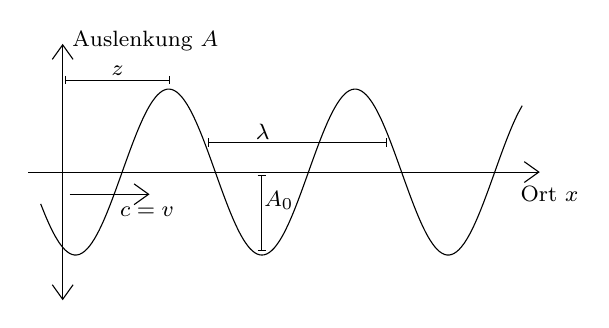
\begin{tikzpicture}[x=0.75pt,y=0.75pt,yscale=-1,xscale=1]
            %uncomment if require: \path (0,209); %set diagram left start at 0, and has height of 209
            % X-Axis
            \draw (42,89.3) -- (288,89.3); % Line
            \draw (281,84.3) -- (288,89.3) -- (281,94.3); % Arrowhead Right
            \draw (278,95) node [anchor=north west][inner sep=0.75pt]  [font=\footnotesize] [align=left] {Ort $x$}; % Text Node x
            
            % Y-Axis
            \draw (58.6,28) -- (58.6,150.6); % Line
            \draw (53.6,35) -- (58.6,28) -- (63.6,35); % Arrowhead Top
            \draw (53.6,143.6) -- (58.6,150.6) -- (63.6,143.6); % Arrowhead Bottom
            \draw (62, 20) node [anchor=north west][inner sep=0.75pt]  [font=\footnotesize]  {Auslenkung $A$}; % Text Node A

            % Sinus
            \draw[color=black, smooth, samples=100, domain=48:280]plot (\x,{cos(+100 + 0.07 * \x r) * 40 + 89.3});
            
            % c = v
            \draw (62,100) -- (100,100); % Line
            \draw (93,95) -- (100,100) -- (93,105); % 
            \draw (85, 105) node [anchor=north west][inner sep=0.75pt]  [font=\footnotesize]  {$c = v$}; % Text Node c

            % z
            \draw (60,45) -- (110,45) (60, 43) -- (60, 47) (110, 43) -- (110, 47); % Line
            \draw (85, 37) node [anchor=north][inner sep=0.75pt]  [font=\footnotesize]  {$z$}; % Text Node z
            
            % lambda
            \draw (129,75) -- (214.5,75) (129, 73) -- (129, 77) (214.5, 73) -- (214.5, 77); % Line
            \draw (155, 65) node [anchor=north][inner sep=0.75pt]  [font=\footnotesize]  {$\lambda$}; % Text Node lambda
            
            % A_0
            \draw (154.5,91) -- (154.5,127) (152.5, 91) -- (156.5, 91) (152.5, 127) -- (156.5, 127); % Line
            \draw (154.5, 103) node [anchor=west][inner sep=0.75pt]  [font=\footnotesize]  {$A_0$}; % Text Node lambda
        \end{tikzpicture}
    \end{center}


    \subsubsection{Gruppengeschwindigkeit $v_g$}
    \begin{minipage}{0.69\linewidth}
        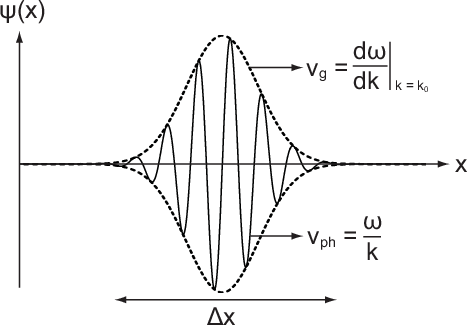
\includegraphics[width = \linewidth]{src/images/gruppengeschwindigkeit.png}
    \end{minipage}
    \begin{minipage}{0.29\linewidth}
        Geschwindigkeit, mit der sich das Wellenpaket fortbewegt
    \end{minipage}
    
    \subsubsection{Reflektion von Wellen}
    Phasensprung bei Welle im Seil mittels Superposition mit einer Welle von der anderen Seite\\
    \begin{minipage}{0.49\linewidth}
        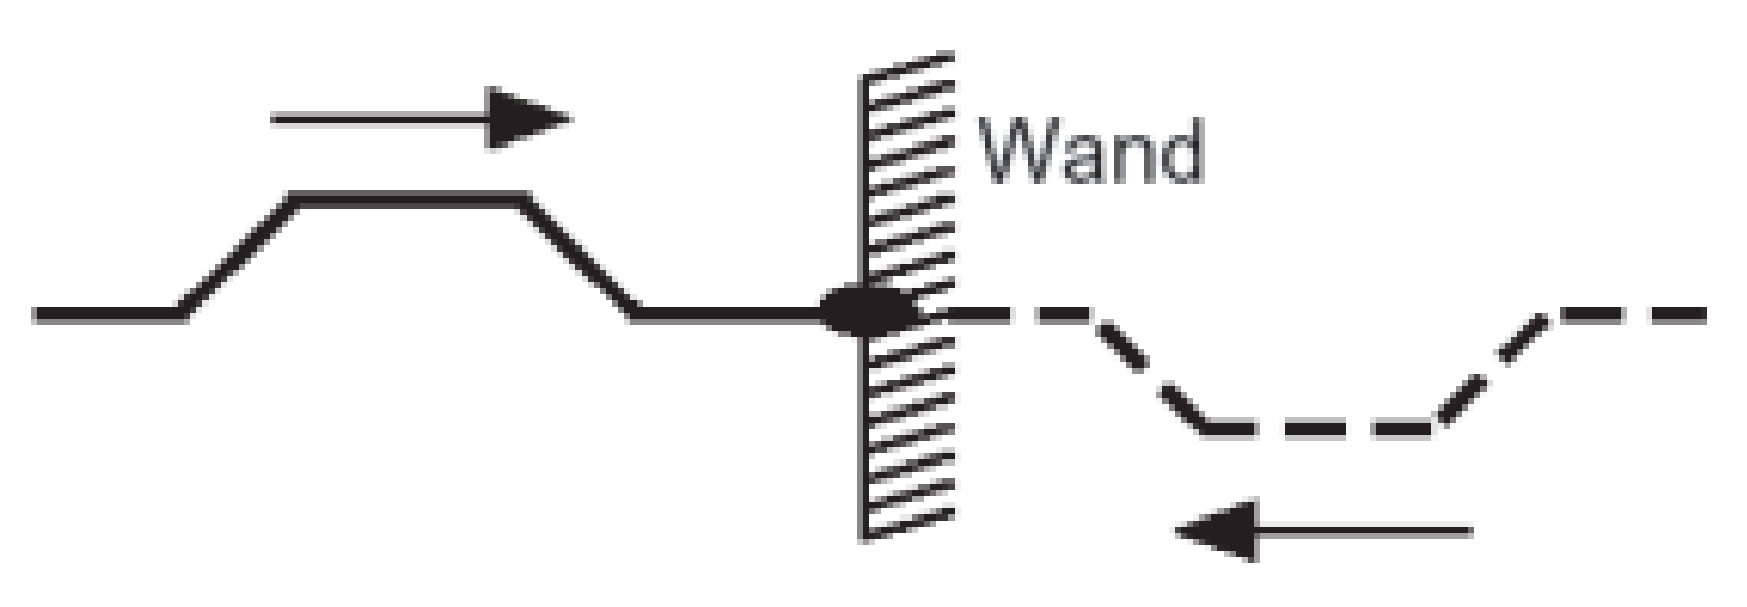
\includegraphics[width = \linewidth]{src/images/welle_superposition_wand.png}
    \end{minipage}
    \begin{minipage}{0.49\linewidth}
        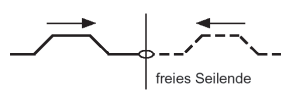
\includegraphics[width = \linewidth]{src/images/welle_superposition_frei.png}
    \end{minipage}

    \subsubsection{Energie von Wellen}

    Intensität einer Welle: Energie
    Potentielle Energie:
    \mathbox{\Delta E_p = \int \vec{F} \vec{dx} = \frac{1}{2} D x_0^2 \text{mit} D = \omega^2 m}
    Kinetische Energie:
    \mathbox{\Delta E_k = \frac{1}{2} \Delta m v^2 \text{mit} v = \omega s}
    $\rightarrow \Delta E_p = \Delta E_k$  

    Energiestromdichte:
    \mathbox{\vec{j_E} = \frac{1}{A} \frac{\Delta E_k}{\Delta t} = \rho_E \vec{v_ph}}